\documentclass[12pt, twoside]{article}
\usepackage[letterpaper, margin=1in, headsep=0.2in]{geometry}
\setlength{\headheight}{0.6in}
%\usepackage[english]{babel}
\usepackage[utf8]{inputenc}
\usepackage{microtype}
\usepackage{amsmath}
\usepackage{amssymb}
%\usepackage{amsfonts}
\usepackage{siunitx} %units in math. eg 20\milli\meter
\usepackage{yhmath} % for arcs, overparenth command
\usepackage{tikz} %graphics
\usetikzlibrary{quotes, angles}
\usepackage{graphicx} %consider setting \graphicspath{{images/}}
\usepackage{parskip} %no paragraph indent
\usepackage{enumitem}
\usepackage{multicol}
\usepackage{venndiagram}

\usepackage{fancyhdr}
\pagestyle{fancy}
\fancyhf{}
\renewcommand{\headrulewidth}{0pt} % disable the underline of the header
\raggedbottom
\hfuzz=2mm %suppresses overfull box warnings

\usepackage{hyperref}

\fancyhead[LE]{\thepage}
\fancyhead[RO]{\thepage \\ Name: \hspace{4cm} \,\\}
\fancyhead[LO]{BECA / Dr. Huson / Geometry\\*  Unit 1: Segments, length, and area\\* 14 Sept 2022}

\begin{document}

\subsubsection*{1.5 Classwork: Equilateral and isosceles triangles, perimeter}
\begin{enumerate}
\item Given $\triangle JKL$ with $\overline{JK} \cong \overline{KL}$. On the diagram mark the congruent line segments with tick marks.
\begin{center}
\begin{tikzpicture}[scale=0.25]
  \draw [thick](0,0)--(9,0)--(4,8)--(0,0);
  \draw [fill] (0,0) circle [radius=0.05] node[below]{$J$};
  \draw [fill] (9,0) circle [radius=0.05] node[below]{$K$};
  \draw [fill] (4,8) circle [radius=0.05] node[above right]{$L$};
\end{tikzpicture}
\end{center}

\item Measure and mark the sides of $\triangle PQR$ in centimeters. Is the triangle scalene, isosceles, or equilateral?
  \begin{center}
  \begin{tikzpicture}[scale=1]
    \draw[thick] (0,0)node[below left]{$P$}--
      (4,0) node[below]{$Q$}--
      (55:4) node[above]{$R$}--cycle;
  \end{tikzpicture}
  \end{center} \bigskip

\item Each of the sides of an equilateral triangle are 8 centimeters long. What is its perimeter? \vspace{1.5cm}

\item The perimeter of rectangle $ABCD$ is 30 inches and its length is twice its width. Fill in the blanks, solve for $x$, and find the rectangle's dimensions.
  \begin{flushright}
    $P = 2x + x + \rule{1.5cm}{0.15mm} + \rule{1.5cm}{0.15mm} = 30$
  \end{flushright}
  \begin{flushleft}
  \begin{tikzpicture}[scale=0.7]
    \draw[thick]
      (0,0)node[below left]{$A$}--
      (6,0)node[below right]{$B$}--
      (6,4)node[above right]{$C$}--
      (0,4)node[above left]{$D$}--cycle;
    \node at (3,-0.8){$2x$ inches};
    \node at (7,2.5){$x$ in};
    \draw (2.9, -0.2)--(2.9,0.2);
    \draw (2.9, 3.8)--(2.9,4.2);
    \draw (-0.2, 1.9)--(0.2, 1.9);
    \draw (-0.2, 2.1)--(0.2, 2.1);
    \draw (5.8, 1.9)--(6.2, 1.9);
    \draw (5.8, 2.1)--(6.2, 2.1);
    \end{tikzpicture}
  \end{flushleft}

\newpage
\item Given point $A(-1)$ as shown below. Locate point, $B > 0$, on the number line such that ${AB}=3 \frac{1}{2}$. \par \smallskip
  \begin{tikzpicture}
    \draw[<->] (-2.5,0)--(6.5,0);
    \foreach \x in {-2,...,6}
      \draw[shift={(\x,0)}] (0pt,-3pt)--(0pt,3pt) node[below=5pt]{$\x$};
    \draw [fill] (-1,0) circle [radius=0.05] node[above] {$A$};
  \end{tikzpicture}
  \begin{enumerate}
    \item Mark and label $B$.
    \item State the value of $B$, writing an equation to support your work.
  \end{enumerate} \vspace{1cm}  

\item Given $M$ is the midpoint of $\overline{AB}$, $AM=5x+11$, $MB=x+21$.
  \begin{enumerate}
    \item Mark the diagram with the values and tick marks
    \item Write an equation and solve for $x$
    \item Check your result
  \end{enumerate} \vspace{1cm}
    \begin{flushleft}
      \begin{tikzpicture}
        \draw [fill] (0,0) circle [radius=0.05] node[below]{$A$};
        \draw [-, thick] (0,0)--(7,0);
        \draw [fill] (3.5,0) circle [radius=0.05] node[below]{$M$};
        \draw [fill] (7,0) circle [radius=0.05] node[below]{$B$};
        %\node at (1.7,0.5) [above]{$x+2$};
        %\node at (5.2,0.5) [above]{$11$};
        %\draw [<->, dashed] (0,-1)--(7,-1);
        %\node at (3.5,-1) [below]{$20$};
      \end{tikzpicture}
    \end{flushleft} \vspace{5cm}

\item The state of Colorado is rectangular in shape. In the north-south direction it runs 280 miles, and east to west 380 miles. Find its perimeter.
  \begin{flushright}
    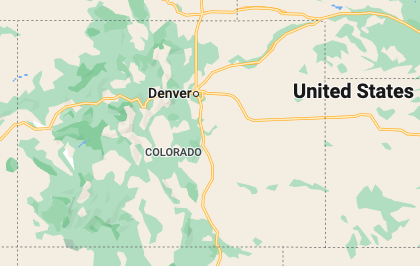
\includegraphics[width=8cm]{../graphics/Colorado.png} \par
    Source: \href{https://www.google.com/maps/@38,-105,6z/}{Google Maps}
  \end{flushright}



\end{enumerate}
\end{document}